% The pathwidth complex -- first full draft (Ralph loop0008 item 08, 2026-10-03).
%
% Build: `make` in this directory (latexmk -pdf). Tables in tables/ are
% generated by `python -m paper2.latex.make_tables`; the bibliography is
% checked by `python -m paper2.latex.check_refs`. See README.md here.
%
% Class: `article`. The INFORMS Journal on Computing class was not obtained:
% INFORMS's author pages refused scripted access on 2026-10-03 (HTTP 403), so
% the template is "to obtain" and the formatting below (one column, 11 pt,
% author-year citations) is a stand-in, not the journal's stated rules.
\documentclass[11pt,letterpaper]{article}

\usepackage[T1]{fontenc}
\usepackage[utf8]{inputenc}
\usepackage{mathptmx}
\usepackage{courier}
\usepackage[protrusion=true,expansion=false]{microtype}
\usepackage[margin=1in]{geometry}
\usepackage{amsmath,amssymb,amsthm}
\usepackage{graphicx}
\usepackage{booktabs}
\usepackage{array}
\usepackage{tabularx}
\usepackage{caption}
\usepackage[section]{placeins}
\usepackage{xcolor}
\usepackage[hyphens]{url}
\usepackage[authoryear,round]{natbib}
\usepackage[colorlinks=true,linkcolor=blue!50!black,citecolor=blue!50!black,urlcolor=blue!50!black]{hyperref}

\graphicspath{{../figures/}}
\numberwithin{figure}{section}
\numberwithin{table}{section}
% Note: natbib labels Yanasse's EJOR paper (the project's "1997b") as 1997a and
% the Pesquisa Operacional paper (the project's "1997a") as 1997b, by title order.
\captionsetup{font=small,labelfont=bf}
\bibliographystyle{plainnat}

% Theorems carry their Lean names in a footnote. \lean{a, b} prints them
% with breaks at the underscores and dots.
\makeatletter
\g@addto@macro{\UrlBreaks}{\do\_\do\.}
\makeatother
\newcommand{\lean}[1]{\footnote{Lean: \path{#1}.}}
\newcommand{\leanfile}[1]{\path{#1}}

\theoremstyle{plain}
\newtheorem{theorem}{Theorem}[section]
\newtheorem{lemma}[theorem]{Lemma}
\newtheorem{proposition}[theorem]{Proposition}
\newtheorem{corollary}[theorem]{Corollary}
\theoremstyle{definition}
\newtheorem{definition}[theorem]{Definition}
\newtheorem{counterexample}[theorem]{Counterexample}
\theoremstyle{remark}
\newtheorem*{remark}{Remark}

\newcommand{\pw}{\mathrm{pw}}
\newcommand{\vs}{\mathrm{vs}}
\newcommand{\ns}{\mathrm{ns}}
\newcommand{\mns}{\mathrm{mns}}
\newcommand{\es}{\mathrm{es}}
\newcommand{\pes}{\mathrm{pes}}
\newcommand{\sbw}{\mathrm{sb}}
\newcommand{\cw}{\mathrm{cw}}
\newcommand{\mcw}{\mathrm{mcw}}
\newcommand{\cl}{\mathrm{cl}}
\newcommand{\Sol}{\mathrm{Sol}}
\newcommand{\cost}{\mathrm{cost}}
\newcommand{\open}{\mathrm{open}}
\newcommand{\close}{\mathrm{close}}
\newcommand{\fin}{\mathrm{fin}}
\newcommand{\pla}{\mathrm{pla}}
\newcommand{\VSG}{\mathrm{VSG}}
\newcommand{\placeholder}[1]{\par\noindent\fbox{\parbox{\dimexpr\linewidth-2\fboxsep-2\fboxrule}{\textbf{Placeholder.} #1}}\par}

\title{The pathwidth complex:\\twelve problems, one width, and a solver proved sound}
\author{Alexandre Linhares\thanks{Draft of 3 October 2026, assembled from the
project's working documents (\texttt{paper2/}). Every number regenerates by the
command named beside it in those documents; the theorems are checked in Lean~4
with Mathlib.}}
\date{Draft, 3 October 2026}

\begin{document}
\maketitle

\begin{abstract}
\noindent\emph{Draft abstract, to be rewritten with Section~\ref{sec:intro}.}
Linhares and Yanasse (2002) listed twelve problems from operations research,
VLSI design and graph theory as equal, up to one, to the minimum number of open
stacks, and gave no proofs. We state each problem precisely and prove what is
true, in Lean: seven of the twelve, and two variants, equal pathwidth or
pathwidth plus one exactly; two lie in bands of width one and two; two are
false as stated. A bibliometric census shows that the literature has settled
on one of the twelve names, pathwidth, and that the communities rarely cite one
another. We then read the exact open-stacks search of Chu and Stuckey (2009) as
a pathwidth algorithm. Two of its published dominance theorems are false; a
14-vertex graph refutes the first, and the same graph refutes its restatement in
Chu's thesis. The repaired rule is an instance of Tamaki's commitment lemma and
costs one bipartite matching per candidate. The whole repaired search is proved
sound in Lean. Run as the default in both of our solvers, it has re-refuted 112 of
the 115 corpus values that rested on the published rules, changing none, and it
emits certificates that an independent checker verifies. The equivalences make one
certified width an answer to every problem in the exact core, and we release
17,714 isomorphism classes from twenty benchmark collections, 16,087 with a
certified pathwidth and a witness layout.
\end{abstract}

% Section 1. Placeholder: waits on the owner's PhD thesis (plan.md, section 1).
\section{Introduction}
\label{sec:intro}

\placeholder{Section~1 waits on the owner's PhD thesis (Linhares, \emph{Industrial
pattern sequencing problems: some complexity results and new local search
models}, 2001), which is not yet held. It is to record how the twelve problems of
Table~1 of \citet{LY2002} were collected, what the thesis proved and what it
only cited, and why the table appeared with no proofs and no graph
(\texttt{paper2/plan.md}, section~1). Kashiwabara and Fujisawa (1979), Table~1's
interval-thickness reference, is still missing.}

\paragraph{The pathwidth complex.} \citet{LY2002} collected, in their
Table~1, twelve problems from operations research, VLSI design and graph theory
that had been studied independently and that compute, on corresponding inputs,
``a function $f(\Pi)$ that is either equal to the number of open stacks or
closely related to it (plus or minus one)'' \citep[p.~1764]{LY2002}. The table
gave references, but no proofs and no graph. Table~\ref{tab:ly2002} reproduces
it as printed. We call this cluster \emph{the pathwidth complex}. Pathwidth is
both the name the literature uses most (Section~\ref{sec:names}) and the
quantity through which every relation in the table is proved
(Section~\ref{sec:equiv}). Of the twelve rows, eight are exactly pathwidth
plus a constant, two lie within a band of width one or two, and two are false
as Table~1 states them (Table~\ref{tab:master}).

\begin{table}[tbp]
\centering
\caption{Display of a family of equivalent problems studied independently on
the literature. Reproduced from \citet[Table~1, p.~1764]{LY2002}, with the
caption, row order and wording as printed; the references are the ones the
original cites, given here by author and year.}
\label{tab:ly2002}
\small
\begin{tabular}{@{}lll@{}}
\toprule
Problem & Discipline & References \\
\midrule
MOSP & Operations research & \citet{Yanasse1997b}; \citet{LY2002ref4} \\
Gate matrix layout & VLSI design & \citet{LY2002ref6}; \citet{LY2002ref8} \\
One-dimensional logic & VLSI design & \citet{LY2002ref7} \\
PLA folding & VLSI design & \citet{LY2002ref6} \\
Interval thickness & Graph theory & \citet{LY2002ref5} \\
Node search game & Graph theory & \citet{LY2002ref9} \\
Edge search game & Graph theory & \citet{LY2002ref10} \\
Narrowness & Graph theory & \citet{LY2002ref11} \\
Split bandwidth & Graph theory & \citet{LY2002ref12} \\
Graph path-width & Graph theory & \citet{LY2002ref13} \\
Edge separation & Graph theory & \citet{LY2002ref14} \\
Vertex separation & Graph theory & \citet{LY2002ref13} \\
\bottomrule
\end{tabular}
\end{table}

\paragraph{Contributions (draft list, for the introduction to argue).}
\begin{itemize}
\item A census of how much each of the twelve names is used, after removing the
  search hits that use the words in other senses; pathwidth has more relevant
  works than the other eleven names together, three times over
  (Section~\ref{sec:names}).
\item Each problem of Table~1 stated as an instance and a question, with the
  graph it lives on and its exact relation to pathwidth, every relation proved
  in Lean; two of Table~1's rows are false as stated (Section~\ref{sec:equiv}).
\item The exact open-stacks search of \citet{ChuStuckey2009} read as a
  vertex-separation search: two of its published dominance theorems are false,
  as are their restatements by \citet{Chu2011} and \citet{Fink2012}; the repair,
  its cost, and a Lean proof that the repaired search is sound; and a proof
  object for its refutations with an independent checker
  (Section~\ref{sec:search}).
\item A dataset of 17,714 isomorphism classes from twenty collections, 16,087 of
  them with a certified pathwidth and a witness layout, which through
  Section~\ref{sec:equiv} answers every problem in Table~1's exact core
  (Section~\ref{sec:dataset}).
\end{itemize}

\paragraph{Notation.} Graphs are finite and simple, $G=(V,E)$, $n=|V|$. A
\emph{layout} is a bijection $L:V\to\{1,\dots,n\}$. For a 0/1 matrix $M$ with
rows $R$ (customers, nets, piece types) and columns $C$ (patterns, gates,
products), the \emph{MOSP graph} $G_M$ has vertex set $R$, with $r\sim r'$ when
some column has a 1 in both rows; each column becomes a clique on its rows. For
an order $\pi$ of the columns, row $r$ is \emph{active} at position $j$ if it
has 1s in columns $x,y$ with $\pi(x)\le j\le\pi(y)$.

% Section 2. Sources: paper2/popularity.md ("For the paper", the method
% paragraph, the sensitivity check), numbers regenerated by
% `python -m paper2.section2_figures --numbers`, figures by
% `python -m paper2.section2_figures`, the table by
% `python -m paper2.latex.make_tables`.
\section{One complex, twelve names}
\label{sec:names}

Table~1 of \citet{LY2002} gathers twelve problems from three disciplines. From
operations research it takes the minimization of open stacks (MOSP); from VLSI
design, gate matrix layout, PLA folding and one-dimensional logic; from graph
theory, pathwidth, vertex separation, interval thickness, node search, edge
search, narrowness, split bandwidth and edge separation. Section~\ref{sec:equiv}
shows which of them are in fact one quantity. This section asks a prior
question: when the literature studies that quantity, which name does it use?
The answer gives the paper its title. Taken together, the problems are one
object seen from three disciplines, and the name the literature has converged
on is pathwidth.

\subsection{Method}
\label{sec:names-method}

We measured how much each name is used with OpenAlex \citep{Priem2022}, on
29 September 2026. For each of the twelve problems we searched titles and
abstracts for its name and its common variants, and restricted the search to
the four fields in which the problems are studied: Computer Science,
Mathematics, Engineering and Decision Sciences. Without that restriction
several names are ordinary words: ``narrowness'' returns over a million works,
and ``edge separation'' returns aerodynamics.

Inside those fields a search hit is still not a work that uses the name.
OpenAlex's search stems words and ignores punctuation, so a quoted phrase
matches more than the phrase. ``Narrowness'' matches ``narrowing'' in term
rewriting; ``node searching'' matches look-ups in peer-to-peer networks;
``split bandwidth'' matches radar interferometry and 5G spectrum assignment;
``path-width'' matches the widths of roads, tool paths and datapaths. We
therefore fetched all 2,271 hits with their titles, abstracts, topics and
venues, and kept a work only if it is about the problem in the sense of
Table~1. For the eleven smaller names the 700 hits were judged one by one. For
pathwidth, the 1,571 hits were filtered by a rule: keep a work that uses the
one-word spelling, that OpenAlex places in a theory subfield, or that mentions
graphs, treewidth or minors and not roads, vehicles, trajectories or datapaths.
We checked the rule by reading samples of what it kept and what it dropped.

The check changed the counts and two of the conclusions. Of the 2,271 hits,
1,593 are relevant: 1,213 for pathwidth and 380 for the other eleven
names.\footnote{OpenAlex returned one pathwidth record twice. The counts are of
records, as the figures draw them; there are 1,212 distinct relevant pathwidth
works, 1,592 in all.} Three names have no relevant work at all. The two
search-game names keep 27\% and 40\% of their hits. MOSP moves from seventh
place to fourth.

The counts are lower bounds. A work can study a problem without naming it in
its abstract, OpenAlex has few abstracts before about 1990, and its citation
counts run below Google Scholar's. The labels were made in one
model-assisted session, record a yes or no per work and not the reason, and
have not been checked by a second labeller. As a second reading we applied a
mechanical rule, the literal phrase with a context term and no exclusion term.
It agrees with the labels on 543 of the 700 labelled works (78\%). Under both
readings pathwidth is more than three times the other eleven names together
(3.2 and 3.6 times), the three empty names stay empty apart from one 5G false
positive, and the search games lose most of their hits. MOSP's rank is the one
conclusion that depends on the reading: fourth under the labels, fifth under
the rule. The labels, the rule, the cached responses and the code that redraws
every figure are in the repository.\footnote{\texttt{paper2/relevance.py},
\texttt{paper2/trends.py}, \texttt{paper2/section2\_figures.py}; regenerate
with \texttt{python -m paper2.section2\_figures}, offline, from the caches of
29 September 2026.}

\subsection{Pathwidth has absorbed the family}

\begin{table}[t]
\centering\small
\caption{Works that use each problem's name in the sense of Table~1, and
citations of the paper Table~1 cites for it. \emph{Relevant}: hits kept by the
check of Section~\ref{sec:names-method}. \emph{Citations}: OpenAlex
\texttt{cited\_by\_count}, 29 September 2026. Kashiwabara and Fujisawa (1979)
has no OpenAlex record. $^{a}$1,212 distinct works.}
\label{tab:names}
% Generated by python -m paper2.latex.make_tables. Source: paper2.section2_figures.numbers() (OpenAlex caches, 2026-09-29).
% Do not edit by hand.
\begin{tabular}{@{}llrrp{4.6cm}r@{}}
\toprule
Problem & Discipline & Relevant & Hits & Reference in the 2002 table & Citations \\
\midrule
Pathwidth & graph theory & 1,213$^{a}$ & 1,571 & \citet{LY2002ref13} & 214 \\
Gate matrix layout & VLSI & 110 & 125 & \citet{LY2002ref6}; \citet{LY2002ref8} & 134 / 89 \\
PLA folding & VLSI & 68 & 74 & \citet{LY2002ref6} & 134 \\
MOSP & operations research & 58 & 60 & \citet{Yanasse1997b}; \citet{LY2002ref4} & 75 / 71 \\
Vertex separation & graph theory & 55 & 100 & \citet{LY2002ref13} & 214 \\
Edge search & graph theory & 38 & 95 & \citet{LY2002ref10} & 293 \\
Node search & graph theory & 34 & 127 & \citet{LY2002ref9} & 124 \\
One-dimensional logic & VLSI & 11 & 18 & \citet{LY2002ref7} & 108 \\
Interval thickness & graph theory & 6 & 10 & \citet{LY2002ref5} & -- \\
Narrowness & graph theory & 0 & 35 & \citet{LY2002ref11} & 44 \\
Split bandwidth & graph theory & 0 & 35 & \citet{LY2002ref12} & 19 \\
Edge separation & graph theory & 0 & 21 & \citet{LY2002ref14} & 77 \\
\midrule
All twelve & & 1,593 & 2,271 & & \\
\bottomrule
\end{tabular}
% check: other eleven = 380; pathwidth distinct = 1212; fetched 2026-09-29, citations 2026-09-29

\end{table}

\begin{figure}[t]
\centering
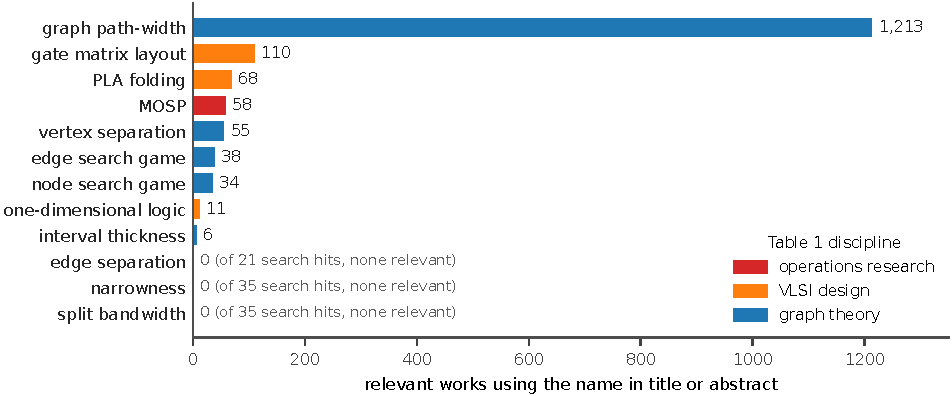
\includegraphics[width=\linewidth]{sec2_fig1_name_usage.pdf}
\caption{Works that use each problem's name, in title or abstract, in the sense
of \citet[Table~1]{LY2002}. OpenAlex, fields Computer Science, Mathematics,
Engineering and Decision Sciences, all years, fetched 29 September 2026. Only
works judged relevant are counted (Section~\ref{sec:names-method}). Colour gives
the discipline that Table~1 assigns the problem. OpenAlex returned one
pathwidth record twice, so pathwidth's 1,213 are 1,212 distinct works.}
\label{fig:names}
\end{figure}

Table~\ref{tab:names} and Figure~\ref{fig:names} give the counts. At 1,213
relevant works pathwidth is 21 times MOSP and more than three times the other
eleven names put together (380). The axis of Figure~\ref{fig:names} is linear
on purpose: the claim is about the size of that gap. Anything one would want to
know about algorithms for this class of problems was most likely published
under ``pathwidth''.

Three of the twelve names are not in use at all, and two more barely.
Narrowness, split bandwidth and edge separation have no relevant work; every
hit was about something else. Split bandwidth is Fomin's own coinage in the
paper Table~1 cites \citep{LY2002ref12}, and nobody adopted it. Interval
thickness (6 works) and one-dimensional logic (11) are nearly as rare. MOSP is
one of the better-used names, at 58 relevant works, behind pathwidth and the two
VLSI layout names.

Citation counts do not track name usage. \citet{LY2002ref10} is the most-cited
paper in the table (293 citations), while only 38 works use ``edge search'' in
its sense: the paper is cited as a foundational result on graph searching, not
because people work on the edge search game under that name. The split is
starker for \citet{LY2002ref7}: 108 citations against 11 works using
``one-dimensional logic''.

\subsection{Three generations}

\begin{figure}[t]
\centering
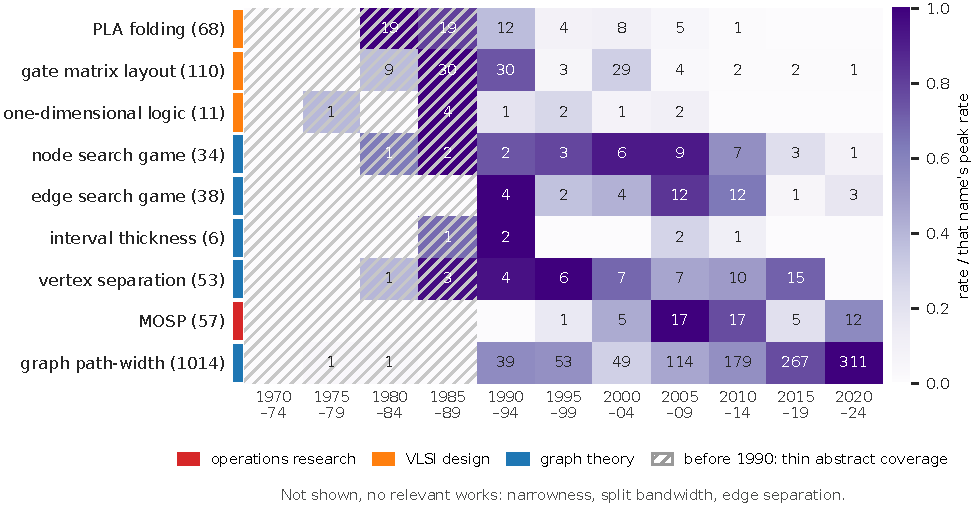
\includegraphics[width=\linewidth]{sec2_fig2_timeline.pdf}
\caption{When each name was in use. The shade is the name's rate, relevant
works per million works in the same four fields in each five-year period, as a
fraction of that name's own peak rate. The numbers are raw counts. Rows are
ordered by the period of their peak. Counts cover 1970--2024, since 2025--26 is
not fully indexed; this is why pathwidth's row totals 1,014 here, against 1,213
in Figure~\ref{fig:names}. Before 1990 (hatched) OpenAlex has few abstracts, so
the early VLSI names are undercounted there.}
\label{fig:timeline}
\end{figure}

Figure~\ref{fig:timeline} shows when each name was alive. The shading is a
rate, so that the growth of publishing as a whole does not make every row
rise, and each row is scaled to its own peak, so that a name with six works
reads as clearly as one with a thousand. The VLSI names belong to the 1980s:
PLA folding and gate matrix layout peak in 1980--89 and fall to almost nothing
after 2010, and one-dimensional logic has no relevant work after 2009. The
graph-searching names peak later and fade. MOSP is the operations-research
generation: it first appears in the 1990s, peaks in 2005--14, and is still
active. Only pathwidth is growing. Its rate has roughly doubled since the 1990s,
from about 15 to 27 works per million, and its 311 relevant works in 2020--24
are more than the whole history of any other name. Rows with a few works per
period move by whole cells on one paper, and should be read as anecdote rather
than trend.

\subsection{Communities that rarely cite each other}

\begin{figure}[t]
\centering
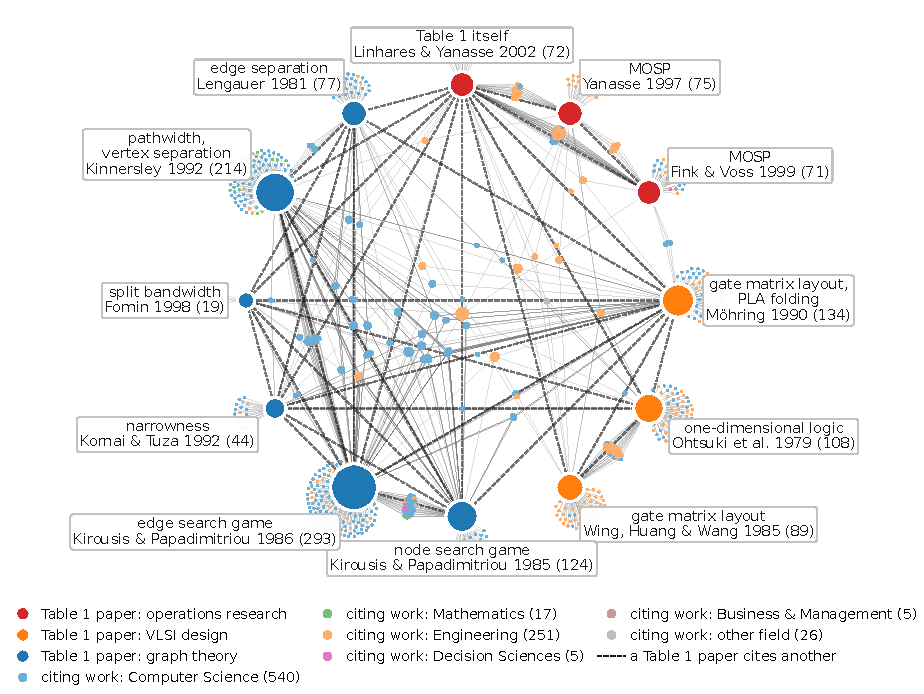
\includegraphics[width=0.92\linewidth]{sec2_fig3_citation_network.pdf}
\caption{The twelve Table~1 papers that OpenAlex indexes, on a circle, sized by
citations (in brackets) and coloured by discipline, and the 844 works that cite
them, coloured by OpenAlex field. 269 of the 844 cite two or more Table~1
papers. 74 of them cite papers of two or more disciplines, counting the eleven
problem papers and not \citet{LY2002} itself, and 63 of those 74 join graph
theory to VLSI. Only 6 cite both a MOSP paper \citep{LY2002ref1,LY2002ref4,LY2002}
and a graph-theory paper. Kashiwabara and Fujisawa (1979) has no OpenAlex
record.}
\label{fig:network}
\end{figure}

Figure~\ref{fig:network} asks whether the three communities read each other.
Works that cite one Table~1 paper ring that paper; works that cite several are
pulled inside the circle. Of the 844 citing works, 269 cite two or more Table~1
papers, but 195 of those stay inside one discipline. 74 span two or more, and
63 of those join graph theory to VLSI. The operations-research side is an
island: only six works cite both a MOSP paper and a graph-theory paper. Two are
by the authors of Table~1; one is MOSP work on graph properties; three are
pathwidth or vertex-separation work from computer science. The fields follow
the disciplines. Works citing the MOSP papers are mostly in Engineering (86 of
135), and works citing the graph-theory papers mostly in Computer Science (417
of 507).

Two consequences shape the rest of the paper. First, a result on any of the
twelve problems should be stated, and searched for, as a result on pathwidth;
Section~\ref{sec:search} does this for an exact MOSP algorithm and finds both a
known theorem it had rediscovered and a published error that the pathwidth
literature's commitment lemma rules out. Second, a benchmark for any problem in the exact
core is a pathwidth benchmark, which is how Section~\ref{sec:dataset} builds its
dataset.

% Section 3. Sources: paper2/problem_transformations.md (problems, statements,
% proofs), paper2/equivalences.md (master table, sources, gaps),
% paper2/proof_reductions.md (faults in published proofs). Lean:
% lean/MOSPFormalization/ and Complex/; axioms printed by paper2/axiom_check.lean.
\section{The equivalences, proved}
\label{sec:equiv}

\citet[p.~1764]{LY2002} introduce Table~1 as ``a set of problems that consist
of, given input $\Pi$, compute a function $f(\Pi)$ that is either equal to the
number of open stacks or closely related to it (plus or minus one)''. The table
cites where each problem was studied. It gives no proofs and no graph. Two
readings of ``plus or minus one'' must be kept apart. Under the \emph{literal}
reading, $f$ lies within one of $Z$, the number of open stacks of the
corresponding instance, on every input. Under the \emph{fixed-offset} reading,
$f = Z + c$ for one constant $c\in\{-1,0,1\}$ on every input. Only the second
makes computing one problem the same as computing another.

This section states each problem as an instance and a question, gives the
relation to pathwidth that is true, and says where it is proved. Every relation
stated below is a theorem of our Lean development unless it says otherwise. All
the theorems named depend only on the axioms \texttt{propext},
\texttt{Classical.choice} and \texttt{Quot.sound}.\footnote{Printed by
\texttt{lake env lean paper2/axiom\_check.lean}, which covers every theorem
named in this paper. The development has one
\texttt{sorry}, a conjecture about lower bounds that no result of this paper
uses.} Table~\ref{tab:master} summarises the result and
Figure~\ref{fig:chain} draws it.

\subsection{The problems}
\label{sec:problems}

Each problem below is a decision problem with an instance and an integer $k$;
its value is the least $k$ for which the answer is yes.

\begin{description}
\item[Pathwidth $\pw(G)$.] Is there a sequence of bags $X_1,\dots,X_r\subseteq V$
  covering $V$, with every edge inside some bag, $X_i\cap X_\ell\subseteq X_j$
  whenever $i\le j\le\ell$, and $|X_i|\le k+1$? \citep[p.~346]{LY2002ref13}.
\item[Vertex separation $\vs(G)$.] Is there a layout $L$ such that for every
  $i<n$ at most $k$ vertices $u$ with $L(u)\le i$ have a neighbour $v$ with
  $L(v)>i$? \citep[p.~346]{LY2002ref13}.
\item[MOSP $Z(M)$.] Given a 0/1 matrix $M$ of customers by patterns, is there
  an order of the patterns with at most $k$ customers active at every position?
  \citep[eqs.~(1)--(2)]{LY2002}.
\item[Gate matrix layout $t(M)$.] Given a net--gate matrix, is there an order of
  the gates and an assignment of nets to $k$ tracks such that nets active at a
  common position get different tracks? \citep[p.~18]{LY2002ref6};
  \citep[Problem~1]{LY2002ref8}.
\item[One-dimensional logic.] Given gates, nets and the nets each gate connects,
  is there an order of the gates whose net intervals have an interval graph of
  clique number at most $k$? Its \emph{connection graph} $H$ joins two nets that
  share a gate. A \emph{boundary} variant pins two gates to the ends
  \citep[\S\S II--IV]{LY2002ref7}.
\item[PLA folding $\pla(M)$.] As gate matrix layout, with at most two nets per
  track. With no such bound (\emph{multiple folding}) it is gate matrix layout
  itself \citep[pp.~25, 36]{LY2002ref6}.
\item[Interval thickness $\theta(G)$.] Is there an interval supergraph of $G$ on
  the same vertices with clique number at most $k$?
  \citep[p.~182]{LY2002ref9}; \citep[p.~31]{LY2002ref6}.
\item[Node search $\ns(G)$.] Can searchers, placed on and removed from vertices,
  clear every edge with at most $k$ on the graph at once, where an edge is
  cleared when both ends are guarded and a clear edge is recontaminated by a
  searcher-free path to a contaminated one? $\mns(G)$ is the same over strategies
  that never recontaminate \citep[p.~181]{LY2002ref9}; \citep[\S2]{LY2002ref10}.
\item[Edge search $\es(G)$.] The same game with a third move, sliding a searcher
  along an edge, which clears that edge; $\pes(G)$ for progressive strategies
  \citep[p.~208]{LY2002ref10}; \citep[p.~53]{EllisSudboroughTurner1994}.
\item[Narrowness $\nu(G)$.] Is there an order $v_1,\dots,v_n$ such that the
  following process never holds more than $k$ vertices: at step $i$ add $v_i$,
  then remove every $v_j$, $j\le i$, with no neighbour $v_\ell$, $\ell>i$?
  \citep[\S2]{LY2002ref11}.
\item[Split bandwidth $\sbw(G)$.] Is there a graph obtained from $G$ by
  repeatedly splitting a vertex into an edge, its neighbours partitioned between
  the two ends, with bandwidth at most $k$? \citep[\S3.2]{LY2002ref12}.
\item[Edge separation.] Table~1 cites \citet{LY2002ref14}, which supports three
  readings: cutwidth $\cw(G)$, the least over layouts of the most edges crossing
  a gap (p.~468); modified cutwidth $\mcw(G)$, counting only edges that pass
  strictly over a vertex (Definition~6); and Lengauer's vertex separator game
  $\VSG(G)$, the least $K$ such that the vertices can be pebbled in an order that
  leaves at most $K$ unpebbled vertices adjacent to pebbled ones (p.~467).
\end{description}

\subsection{What is true}

\begin{table}[t]
\centering\small
\caption{Table~1 of \citet{LY2002}, settled. \emph{Relation}: what is true and
proved in Lean, on the graph the problem lives on (the MOSP graph or net graph
for the matrix problems, the input graph otherwise). \emph{Status}:
\emph{exact}, a fixed offset; \emph{band}, an inequality whose ends both occur;
\emph{false}, Table~1's claim fails, with a counterexample family proved in
Lean.}
\label{tab:master}
\begin{tabularx}{\linewidth}{@{}>{\raggedright}p{2.7cm}>{\raggedright}p{3.4cm}>{\raggedright\arraybackslash}X l@{}}
\toprule
Problem & Proved in & Relation & Status \\
\midrule
MOSP & \citet{Yanasse1997a}; \citet{FellowsLangston1989}; \citet{LY2002} &
  $Z(M)=\pw(G_M)+1$ ($M$ has a 1) & exact \\
Gate matrix layout & \citet{LY2002ref6} & $t(M)=Z(M)=\pw(G_M)+1$ & exact \\
One-dim.\ logic & \citet{LY2002ref7} & tracks $=\theta(H)=\pw(H)+1$; boundary variant $\ge\pw(H)+1$ & exact \\
PLA folding & \citet{LY2002ref6} & $\max(\pw+1,\lceil|N|/2\rceil)\le\pla$, gap unbounded; multiple folding $=\pw+1$ & false; variant exact \\
Interval thickness & \citet{LY2002ref6}; \citet{LY2002ref9} & $\theta=\pw+1$ ($V\ne\emptyset$) & exact \\
Node search & \citet{LY2002ref9,LY2002ref10}; \citet{BienstockSeymour1991} & $\ns=\mns=\vs+1=\pw+1=\theta$ ($E\ne\emptyset$) & exact \\
Edge search & \citet{EllisSudboroughTurner1994}; \citet{LY2002ref10} & $\vs\le\es\le\vs+2$, also for $\pes$ & band \\
Narrowness & \citet{LY2002ref11} & $\nu=\pw+1$ ($V\ne\emptyset$) & exact \\
Split bandwidth & \citet{LY2002ref12} & $\pw\le\sbw\le\pw+1$ & band \\
Path-width & \citet{LY2002ref13} & the reference & definition \\
Edge separation & \citet{LY2002ref14} & $\cw,\mcw$ unbounded against $\pw$ (stars); $\VSG=\max(1,\vs)$ & false; VSG exact \\
Vertex separation & \citet{LY2002ref13} & $\vs=\pw$ & exact \\
\bottomrule
\end{tabularx}
\end{table}

\begin{figure}[t]
\centering
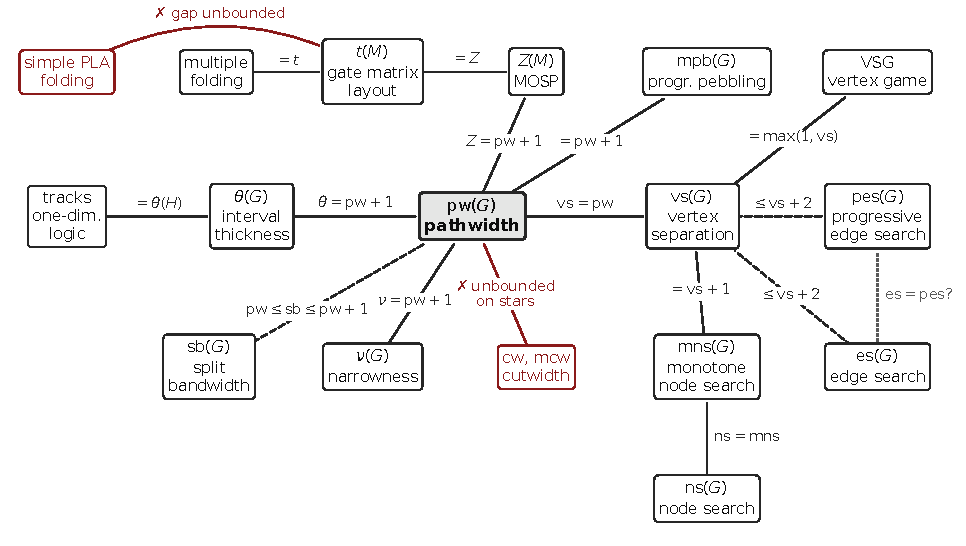
\includegraphics[width=\linewidth]{sec3_fig1_chain}
\caption{The equivalences of Table~\ref{tab:master} as a graph around
pathwidth. Solid edges are exact relations, dashed edges bands, both proved in
Lean; the dotted edge is LaPaugh's $\mathrm{es}=\mathrm{pes}$, the one relation
not proved, which no row needs. Dark red marks Table~1's two false claims, each
refuted by a counterexample family proved in Lean. The four matrix problems (top
left) live on the MOSP graph $G_M$ or the net graph $H$; $\mathrm{mpb}$ is the minimum
progressive pebbling number of Section~\ref{sec:thirteenth}. Hypotheses are
omitted: $M$ has a 1, $V\neq\emptyset$, or $G$ has an edge, as in
Table~\ref{tab:master}. Two edges that follow from the others,
$\mathrm{mns}=\theta$ and $\mathrm{ns}=\mathrm{vs}+1$, are not drawn.}
\label{fig:chain}
\end{figure}

Two lemmas carry most of the exact rows. For a path decomposition and a vertex
$v$, let $\mathrm{first}(v)$ and $\mathrm{last}(v)$ be the least and greatest
indices of bags containing $v$; the decomposition's interval property says
$v\in X_i$ exactly when $\mathrm{first}(v)\le i\le\mathrm{last}(v)$.

\begin{lemma}[Helly for intervals]\label{lem:helly}
Pairwise intersecting intervals of a line have a common point.
\end{lemma}
\begin{proof}
Let $a$ be the largest left end. Any two intervals meet, so every right end is
at least every left end, and in particular at least $a$. So $a$ lies in all of
them.
\end{proof}

\begin{lemma}[cliques sit in a bag]\label{lem:clique}
In a path decomposition of $G$, every clique of $G$ lies inside one bag.\lean{PathDecomposition.exists_bag_of_isClique}
\end{lemma}
\begin{proof}
The bags containing a vertex $u$ of the clique form the interval
$[\mathrm{first}(u),\mathrm{last}(u)]$. Two vertices of the clique are
adjacent, so their edge lies in a bag and their intervals meet. By
Lemma~\ref{lem:helly} all the intervals share an index $i$, and the clique lies
in $X_i$.
\end{proof}

\begin{theorem}[vertex separation is pathwidth]\label{thm:vs}
For every graph, $\vs(G)=\pw(G)$.\lean{vertexSeparation_eq_pathwidth}
\end{theorem}
This is Theorem~3.1 of \citet{LY2002ref13}. From a layout $L$ of separation $k$,
the bags $X_i = V_L(i-1)\cup\{L^{-1}(i)\}$, where $V_L(i)$ is the set the
definition counts, form a decomposition of width $k$. Conversely, ordering the
vertices by $\mathrm{first}$ gives a layout in which everything counted at a cut
lies in the bag where the next vertex first appears, beside that vertex.

\begin{theorem}[MOSP is pathwidth plus one]\label{thm:mosp}
If $M$ has at least one 1, then $Z(M)=\pw(G_M)+1$.\lean{MOSPInstance.mospValue_eq_pathwidth_add_one}
\end{theorem}
\begin{proof}
($\le$) Take a decomposition of $G_M$ of width $k$. The rows of each column form
a clique, so by Lemma~\ref{lem:clique} they lie in a bag $X_{b(c)}$. Order the
columns by $b(c)$. If row $r$ is active at the position of column $c$, it has
columns $x,y$ with $b(x)\le b(c)\le b(y)$, and $r\in X_{b(x)}\cap X_{b(y)}$, so the
interval property gives $r\in X_{b(c)}$. At most $k+1$ rows are active there.

($\ge$) Take an order with at most $Z$ active rows at every position. The
active sets, with a singleton bag for each row with no 1, form a path
decomposition: rows sharing a column are both active at its position, and a row
is active on an interval of positions. Its width is $Z-1$, using $Z\ge1$.
\end{proof}

Read as a cutting problem, Theorem~\ref{thm:mosp} is Proposition~5 of
\citet{Yanasse1997a}, which turns each pattern into a clique on its piece types;
read as a layout problem, it is Theorem~7 of \citet{FellowsLangston1989}, with
the column-expansion Lemma~4.1 of \citet{FellowsLangston1987}; and
\citet[Prop.~2]{LY2002} identify MOSP with gate matrix layout. The proof above
needs the Helly property and the interval property, not Hall's theorem. It needs
no assumption that the instance is reduced.

The graph matters. The pattern graph, with the patterns as vertices joined when
they share a customer, gives no bound in either direction: one pattern shared by
four customers who each have a private pattern has $Z=4$, while its pattern
graph is the star $K_{1,4}$, of pathwidth~1.\lean{star_mospValue, star_pathwidth_agreementGraph, star_refutes_pattern_graph_bound} A single
customer with many patterns errs the other way.

The other exact rows attach to Theorems~\ref{thm:vs} and~\ref{thm:mosp}.

\begin{theorem}[the exact core]\label{thm:core}
\leavevmode
\begin{enumerate}
\item Gate matrix layout is MOSP on the same matrix: if $M$ has a 1,
  $t(M)=Z(M)=\pw(G_M)+1$. For a fixed gate order the fewest tracks equals the
  most nets active at one position, by the left-edge algorithm.\lean{NetGateMatrix.tracks_eq_mospValue, NetGateMatrix.tracks_eq_pathwidth_add_one}
\item Interval thickness: if $V\ne\emptyset$, $\theta(G)=\pw(G)+1$
  \citep[Prop.~3.5]{LY2002ref6}.\lean{intervalThickness_eq_pathwidth_add_one}
\item One-dimensional logic: if every net lies on a gate, the fewest tracks is
  $\theta(H)$, and if some gate connects a net it is $\pw(H)+1$
  \citep[Thm~3]{LY2002ref7}.\lean{LogicArray.tracks_eq_intervalThickness, LogicArray.tracks_eq_pathwidth_add_one}
\item Narrowness: if $V\ne\emptyset$, $\nu(G)=\pw(G)+1$, and for each order
  $\sigma$, $\nu(\sigma)=\vs(\sigma^{\mathrm{rev}})+1$
  \citep[Prop.~3.1]{LY2002ref11}.\lean{narrowness_eq_pathwidth_add_one}
\item Node search: for every graph $\ns(G)=\mns(G)$, and if $E\ne\emptyset$,
  $\ns(G)=\vs(G)+1=\pw(G)+1=\theta(G)$
  \citep[Thm]{LY2002ref9}; \citep[Thms~2.3, 4.1]{LY2002ref10}.\lean{nodeSearchMonotonicity, nodeSearch_eq_vertexSeparation_add_one, nodeSearch_chain}
\item Multiple folding: the fewest tracks is $t(M)=\pw(G_M)+1$
  \citep[Thm~3.14]{LY2002ref6}.\lean{NetGateMatrix.foldTracks_eq_pathwidth_add_one}
\item Lengauer's vertex separator game: $\VSG(G)=\max(1,\vs(G))$
  \citep[Thm~4]{LY2002ref14}.\lean{vsg_eq_max}
\end{enumerate}
\end{theorem}

The Lean proof that node search is monotone follows the crusade argument of
\citet{BienstockSeymour1991}, not the reduction to edge search of
\citet{LaPaugh1993} on which \citet{LY2002ref10} rely.

\begin{theorem}[bands]\label{thm:bands}
For every graph, $\pw(G)\le\sbw(G)\le\pw(G)+1$ \citep[Thm~8]{LY2002ref12}, and
$\vs(G)\le\es(G)\le\vs(G)+2$, and the same for $\pes$
\citep[Thm~2.1]{EllisSudboroughTurner1994}.\lean{pathwidth_le_splitBandwidth_le_pathwidth_add_one, vertexSeparation_le_edgeSearch_le_add_two, vertexSeparation_le_progressiveEdgeSearch_le_add_two}
\end{theorem}
Every end of both bands occurs. $K_2$ has $\sbw=\pw=1$ and $\es=\vs=1$; the star
$K_{1,3}$ has $\pw=1$ and $\sbw=2$, and $\vs=1$ with $\es=2$; and $K_{3,3}$ has
$\vs=3$ with $\es=5$. These values come from a brute-force check of every
quantity from its own definition, not from Lean.\footnote{\texttt{python -m
paper2.complex\_check}; $\sbw(K_{1,3})\ge2$ is also argued by hand: splits of a
tree are trees and keep at least three leaves.} Fomin assumes a connected graph
with at least two vertices; the Lean proof needs neither. The equality
$\es=\pes$ \citep{LaPaugh1993} is stated in Lean as a named proposition and used
by no row.

\begin{theorem}[two rows are false]\label{thm:false}
\leavevmode
\begin{enumerate}
\item PLA folding: for a matrix with a 1,
  $\max(\pw(G_M)+1,\lceil|N|/2\rceil)\le\pla(M)$, and the gap to $\pw+1$ is
  unbounded. The $5\times5$ identity needs 3 tracks while $\pw(G_M)+1=1$, and the
  path $P_n$ as a matrix, one gate per edge, has $t=2$ and
  $\pla\ge\lceil n/2\rceil$, so the gap is unbounded on connected instances too
  \citep[Prop.~3.15]{LY2002ref6}.\lean{plaTracks_idMatrix_five, plaTracks_idMatrix_unbounded, plaTracks_pathMatrix_unbounded}
\item Edge separation read as cutwidth: $\pw\le\cw$ always, but
  $\cw(K_{1,n})\ge n/2$ and $\mcw(K_{1,n})\ge n/2-1$ while $\pw(K_{1,n})=1$; so
  neither cutwidth reading is within a constant of pathwidth.\lean{cutwidth_unbounded, modCutwidth_unbounded}
\end{enumerate}
\end{theorem}
Table~1's PLA claim holds for multiple folding (Theorem~\ref{thm:core}). The
edge-separation row is also misattributed: what \citet{LY2002ref14} proves
exactly is the vertex separator game, which is Table~1's vertex separation row.

\subsection{Edge cases and a gap in a published proof}

Three of the published equalities fail on degenerate inputs, and each failure
is proved in Lean. On a nonempty graph with no edges, $\ns=0$ while
$\vs+1=\theta=1$, so both equalities of \citet{LY2002ref9,LY2002ref10} need an
edge.\lean{nodeSearch_ne_intervalThickness_of_edgeless, monotoneNodeSearch_ne_vertexSeparation_add_one_of_edgeless}
For a matrix with no 1s, $Z=0$ while $\pw+1=1$. Lengauer's Theorem~4 fails at
$K=0$ on an edgeless graph.\lean{isPositiveVSG_triangleGraph_counterexample}
\citet[Thm~3.9]{LY2002ref6}, $t=\ns$, fails literally on the $1\times1$ matrix
$[1]$.\lean{tracks_ne_monotoneNodeSearch_one}

The published proof of $\vs\le\ns-1$ \citep[Thm~4.1]{LY2002ref10} has a gap. It
orders the vertices by when they first receive a searcher and claims that every
vertex counted at the worst cut still holds a searcher, ``since the vertices in
$D_{i_0}$ are joined to vertices not yet cleared'' (p.~217). A strategy may place
a searcher and remove it again before clearing anything, which recontaminates
nothing. On $K_{1,3}$, placing and removing a searcher on each leaf before
guarding the centre is an optimal recontamination-free strategy for which the
claim fails.\lean{kirousisPapadimitriou_claim2_false} The theorem is true. The
repair orders the vertices by clearing time, as our Lean proof does, or uses the
paper's own normal form, its Corollary~2.4.

\subsection{A thirteenth member}\label{sec:thirteenth}

Progressive black-white pebbling, which is not in Table~1, belongs to the exact
core. \citet[Thm~3]{LY2002ref14} gives
$\vs(G)\le K\iff\mathrm{pbw}(G_d)\le K+2$ on the dag $G_d$ built from $G$; his
Theorem~2 gives $\mathrm{pbw}(D)=\vs(D_u)+1$ on a dag $D$, where $D_u$ is the
MOSP graph of the matrix whose column $v$ is $v$ with its predecessors; and the
minimum progressive pebbling number of \citet[Thm~3.1]{LY2002ref10} equals
$\pw+1$. All three are proved in Lean, each with its hypothesis: Lengauer's
Theorem~2 in its instance form fails at $K=1$ on a dag with no arcs, and
$\mathrm{mpb}=\ns$ fails on edgeless graphs.\lean{pbw_lengauerD_eq_pathwidth, pbw_eq_mospValue_pebbleMatrix, mpb_eq_pathwidth_add_one}

\paragraph{Summary.} Seven of Table~1's twelve problems are pathwidth, or
pathwidth plus one, exactly: MOSP, gate matrix layout, one-dimensional logic,
interval thickness, node search, narrowness and vertex separation, with pathwidth
itself as the reference. So are two variants, multiple folding and Lengauer's
vertex separator game. Split bandwidth and edge search are bands of width one
and two, which meet the literal reading of Table~1 and not the fixed offset.
Simple PLA folding and edge separation are false as stated. One theorem is
stated and not proved, LaPaugh's $\es=\pes$, and no row needs it. One of
Table~1's references, Kashiwabara and Fujisawa (1979), is not held; its row is
proved from \citet{LY2002ref6} and \citet{LY2002ref9}.

% Section 4. Sources: paper2/revised_algorithm.md (4.1-4.7), search_soundness.md,
% solver_fix.md (cost, re-certification), prior_art_counterexample.md (prior
% art), certificates.md (proof object), dataset.md (the dataset). Lean:
% lean/MOSPFormalization/Search/. Tables from tables/ (make_tables.py).
% Page numbers for Chu & Stuckey (2009) are those of the preprint
% literature/chu_stuckey_2009.pdf; for Chu (2011) the printed ones.
\section{An exact open-stacks search, read as a pathwidth solver}
\label{sec:search}

The best exact method for MOSP on the standard benchmarks is the \emph{customer
search} of \citet{ChuStuckey2009}. It searches over the orders in which the
customers' stacks close, not over product sequences, and prunes with dominance
rules, three of them stated as theorems (their Theorems~1, 2 and~3) and a fourth,
the subset rule, in their \S2. \citet{ChuStuckey2009} place MOSP among ``graph
path-width and gate matrix layout'', citing \citet{LY2002}, but do not use
pathwidth in the search. By Theorem~\ref{thm:mosp} it is nevertheless a
pathwidth algorithm: any graph is the MOSP graph of the instance with one
customer per vertex and one product per edge, whose optimum is pathwidth plus
one.

This section reads the search that way, and finds three things. Two of the
published theorems are false, and so are their restatements in Chu's thesis
\citep{Chu2011} and, with a stronger premise, in \citet{Fink2012}. The repaired
first rule is an instance of a known pathwidth theorem, Tamaki's commitment
lemma; the published rule is that lemma with its interior condition dropped. And
the whole repaired search is proved sound in Lean. All Lean names in this
section are in \leanfile{lean/MOSPFormalization/Search/}, which has no
\texttt{sorry} and the standard axioms only.

\subsection{The search decides pathwidth}
\label{sec:search-def}

\citet[p.~4]{ChuStuckey2009} observe that the products matter only through the
MOSP graph. So fix a graph $G=(C,E)$ on the customers and an integer $k\ge0$.
For a customer $c$ and a set $T\subseteq C$ of closed customers, write
$N[c]$ for the closed neighbourhood of $c$, and
\begin{align*}
O(T) &= \textstyle\bigcup_{c\in T}N[c] && \text{the stacks opened once $T$ has closed},\\
\fin(X) &= \{c : N[c]\subseteq X\} && \text{the customers free to close when $X$ is open},\\
\cl(T) &= \fin(O(T)) && \text{the \emph{free closure} of $T$},\\
b(T) &= |O(T)\setminus T| && \text{the stacks open after $T$ has closed},\\
o(c,T) &= N[c]\setminus O(T),\quad \open(c,T)=|o(c,T)| && \text{the stacks closing $c$ would newly open.}
\end{align*}
A \emph{move} at $T$ closes one customer $c\notin T$, at cost
$\cost(T,c)=|O(T\cup\{c\})\setminus T| = b(T\cup\{c\})+1$, the stacks open at
that moment counting $c$; it is \emph{playable} when $\cost(T,c)\le k$. Write
$P_k(T)$ when some order of $C\setminus T$ has every step playable. On entering
a node the search closes every free customer, so it stands only at
\emph{states}, sets with $S=\cl(S)$, and the \emph{child} of $S$ by $c$ is
$S\cdot c=\cl(S\cup\{c\})$. The search's predicate $\Sol_k(S)$ holds when $S=C$,
or when some playable $c$ has $\Sol_k(S\cdot c)$.\lean{stepCost, Solvable, SearchSol}
Every node the search visits satisfies the invariant $b(S)\le k$.

\begin{lemma}[free moves never hurt]\label{lem:F}
If $b(T)\le k$, then $P_k(T)\iff\Sol_k(\cl(T))$.\lean{solvable_iff_searchSol_cl}
\end{lemma}
Closing a customer whose neighbourhood is open opens nothing, never makes a
later step dearer, and leaves one fewer stack open. The hypothesis is needed:
closing the free customers one by one costs $b(T)$ at each step.

\begin{theorem}[the search decides pathwidth]\label{thm:decides}
For nonempty $C$, $\Sol_k(\emptyset)\iff\pw(G)+1\le k$; on the MOSP graph of an
instance $M$ with a requirement, $\Sol_k(\emptyset)\iff Z(M)\le k$.\lean{searchSol_empty_iff_pathwidth_add_one_le, searchSol_mospGraph_iff_mospValue_le}
\end{theorem}
\begin{proof}
For a closing order $c_1,\dots,c_n$ with prefixes $S_i$, the $i$-th step costs
$1+|\partial S_i|$, where $\partial X$ is the set of vertices outside $X$ with a
neighbour in $X$. Read backwards as a layout, the cut separating $C\setminus S_i$
from $S_i$ counts exactly $\partial S_i$. So the cost of the order is the vertex
separation of the reversed layout plus one, and Lemma~\ref{lem:F} at the root and
Theorem~\ref{thm:vs} finish the proof. The Lean statement goes through
narrowness \citep{LY2002ref11}, which counts the forward order directly.
\end{proof}

So a refutation, $\neg\Sol_k(\emptyset)$, may only mean $\pw(G)>k-1$. The rest
of the section asks whether the pruning rules preserve that meaning.

\paragraph{What a rule must satisfy.} At a state $S$ the search has a set $Q$ of
\emph{old moves} (Section~\ref{sec:other-rules}). Its candidates are the
customers outside $S\cup Q$; the \emph{cost cut} keeps the playable ones, $P$,
in index order, and a \emph{filter} keeps a sublist $L\subseteq P$. The filter
is \emph{node-sound} at $(S,Q)$ if, whenever every $q\in Q$ has
$\neg\Sol_k(S\cdot q)$, $\Sol_k(S)$ implies $\Sol_k(S\cdot c)$ for some $c\in L$.\lean{NodeSoundAt}
Each rule justifies a discarded move $r$ by a \emph{covering}, a move $c$ with
$\Sol_k(S\cdot r)\Rightarrow\Sol_k(S\cdot c)$. A node is sound when every link a
rule cites is a true covering and every chain of links from a discarded
candidate ends in $L$ or in $Q$; the second condition can fail through a cycle
even when every link is true. The filter runs the definite move, then the subset
rule, then the better move, each once.

\subsection{The definite move is false as published}
\label{sec:definite}

\citet[\S3.1, p.~6]{ChuStuckey2009} state:
\begin{quote}
\textbf{Theorem 1.} Suppose S ++ [q] is playable and close(q, S) $\ge$
open(q, S), then if U$'$ = S ++ R is a solution, there exists a solution
U = S ++ [q] ++ R$'$,
\end{quote}
where $\close(q,S)$ counts the customers $d$ with $o(d,S)\subseteq o(q,S)$
(p.~4). The rule keeps $q$ alone. We read $d$ as ranging over customers not yet
closed, as the code does; read literally, closed customers count too, which
weakens the premise, and both readings are refuted below. \citet[Thm~6.3.6,
p.~142]{Chu2011} restates the theorem with the same premise and proof, reworded
for $k$ stacks. Write $X=S\cdot q$.

\begin{lemma}[what the premise says]\label{lem:premise}
$\close(q,S)=|X\setminus S|$. Hence the premise holds iff $b(X)\le b(S)$: the
child has no more open stacks than the parent.\lean{closeCount_eq, isDefinite_iff}
\end{lemma}

\begin{figure}[t]
\centering
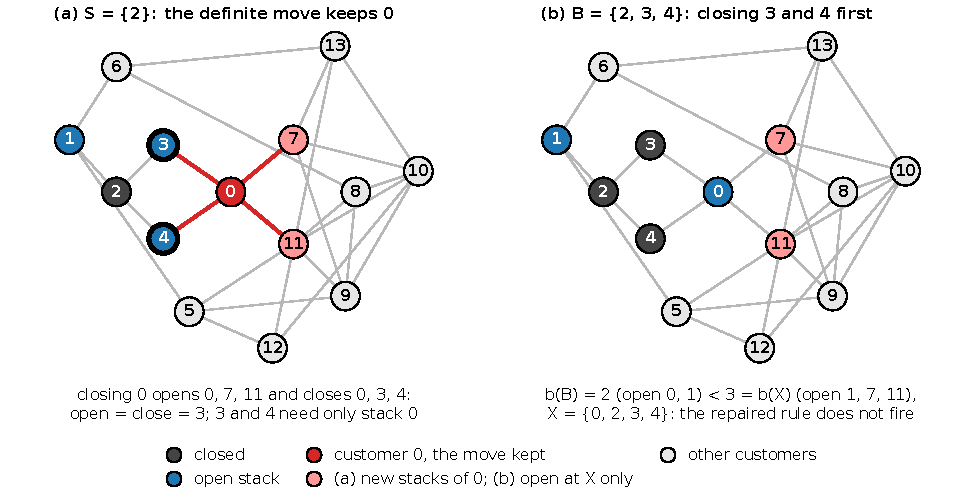
\includegraphics[width=0.85\linewidth]{definite_counterexample.pdf}
\caption{The graph of Counterexample~\ref{cex:definite} at the state where the
definite move fails. Customer 2 is closed; 1, 3 and 4 are open. Moving 0 opens
the new stacks 0, 7 and 11 and closes 0, 3 and 4, so open = close = 3 and the
rule keeps 0 alone. But 3 and 4 have the single new stack 0 between them:
closing them first gains two stacks for the price of one, which a solution
starting with 0 cannot match. Regenerate with \texttt{python -m
paper2.counterexample\_figure}, which recomputes every labelled fact.}
\label{fig:cex}
\end{figure}

\begin{counterexample}\label{cex:definite}
Let $G$ be the graph on customers $0,\dots,13$ with the 26 edges
\begin{gather*}
0\text{--}3,\ 0\text{--}4,\ 0\text{--}7,\ 0\text{--}11,\ 1\text{--}2,\ 1\text{--}5,\ 1\text{--}6,\ 2\text{--}3,\ 2\text{--}4,\ 5\text{--}9,\ 5\text{--}11,\ 5\text{--}12,\ 6\text{--}8,\\
6\text{--}13,\ 7\text{--}9,\ 7\text{--}10,\ 7\text{--}13,\ 8\text{--}9,\ 8\text{--}10,\ 8\text{--}11,\ 9\text{--}10,\ 9\text{--}11,\ 10\text{--}11,\ 10\text{--}12,\ 10\text{--}13,\ 12\text{--}13,
\end{gather*}
with $S=\{2\}$, $k=6$ and $q=0$ (Figure~\ref{fig:cex}). Then $O(S)=\{1,2,3,4\}$,
$o(0,S)=\{0,7,11\}$ and $\cost(S,0)=6$, so $0$ is playable; the customers with
$o(d,S)\subseteq\{0,7,11\}$ are $0$, $3$ and $4$, so $\close(0,S)=3\ge\open(0,S)$;
and $0$ comes first in index order, so the rule keeps only $0$. A solution
exists from $S$: the order
\[1,3,4,6,12,13,0,5,7,8,9,10,11\]
costs at most 6. None exists
from the child $X=\{0,2,3,4\}$: only seven sets are reachable from $X$ by moves
of cost at most 6, and none is $C$.\lean{definiteMove_counterexample, cexFamily_closed}
\end{counterexample}

The published implication, as a universal statement, is refuted in Lean under
both readings of $\close$, and so is the thesis's Theorem~6.3.6.\lean{chuStuckey_theorem1_false, chuStuckey_theorem1_false_literal, chuThesis_theorem636_false}
The smallest graph on which the rule loses the last solution has 14 customers:
there is none on any graph to 9 vertices, by exhaustion, and none on the 88,802
connected graphs on 10 vertices with at most 14 edges. The counterexample was
found by a search over a family of gadgets built from the failed proof, and
minimised by deletion. \citet[pp.~27--28]{Fink2012} restates the rule with a
stronger premise, counting only dominated customers of smaller index than $q$.
The graph above refutes it under no labelling, but a third twin of 3 and 4 gives
a 15-customer graph that does.\lean{fink_theorem1_false}

\paragraph{Why the published proof fails.} The proof moves $q$ to the front of a
solution and claims that after each prefix ``we have at most open(q, S) extra
stacks open, but at least close(q, S) extra stacks closed'' (p.~6). At a prefix
$T\supseteq S$ that does not yet contain $q$, moving $q$ forward changes the open
stacks by $b(T\cup X)-b(T) = |N[q]\setminus O(T)|-|X\setminus T|$. At $T=S$ this
is $\open-\close\le0$. But customers of $X$ that the solution has \emph{already}
closed are in $T$ and no longer count as extra stacks closed, while the stacks
$q$ opens may still be new. In the example, a solution may begin with 3, after
which 4 is free: at $T=\{2,3,4\}$, moving 0 forward costs one more stack. A
second, independent slip: even where the conclusion holds, the literal sequence
$S \mathbin{+\!\!+} [q] \mathbin{+\!\!+} R'$ need not be a solution, because a
customer that $q$ frees stays open until its turn; the argument needs the free
moves.

\paragraph{The repair.} Call $q$ \emph{hereditarily definite} at $S$ when
$b(X)\le b(B)$ for every $B$ with $S\subseteq B\subseteq X$ and $q\notin B$. By
Lemma~\ref{lem:premise}, the published premise is the case $B=S$. In the
counterexample the repair fails at $B=\{2,3,4\}$, where $b(B)=2<3=b(X)$.\lean{IsHereditarilyDefinite, not_isHereditarilyDefinite_cex}

\begin{lemma}[open stacks are submodular]\label{lem:submod}
For all $A,B\subseteq C$, $b(A\cup B)+b(A\cap B)\le b(A)+b(B)$.\lean{openStacks_submodular}
\end{lemma}
\begin{proof}
$b(T)=|O(T)|-|T|$, $O(A\cup B)=O(A)\cup O(B)$ and $O(A\cap B)\subseteq
O(A)\cap O(B)$; the customers themselves balance exactly.
\end{proof}

\begin{theorem}[the repaired definite move is sound]\label{thm:repaired}
If $q\notin S$ is hereditarily definite at $S$, then $P_k(S)\Rightarrow P_k(X)$.
At a state with the invariant, $\Sol_k(S)\Rightarrow\Sol_k(S\cdot q)$.\lean{solvable_cl_insert_of_hereditarilyDefinite, searchSol_cl_insert_of_hereditarilyDefinite}
\end{theorem}
\begin{proof}
Take an order from $S$ of cost at most $k$ with prefixes $T_i$, in which $q$ is
the $j$-th step, and follow it from $X$, skipping customers already in $X$. A
step $i<j$ closes $c_i$ at $T_{i-1}\cup X$. With $Z=T_i$ we have
$S\subseteq Z\cap X\subseteq X$ and $q\notin Z$, so the hypothesis gives
$b(X)\le b(Z\cap X)$, and Lemma~\ref{lem:submod} gives $b(Z\cup X)\le b(Z)$: the
step costs no more than the original. After step $j-1$ the closed set contains
$T_j$ with the same opened set, and the rest of the order applies. The search's
form follows by Lemma~\ref{lem:F}.
\end{proof}

This theorem is not new. The hereditary premise is the commitment condition of
Tamaki, and the proof is the proof of the commitment lemma,
\citet[Lemma~1, p.~142]{Kitsunai2016}; Section~\ref{sec:layouts} makes the
correspondence exact. What we did not find in the papers we hold is the
following cheap form of the test.

\begin{theorem}[the repair is a matching condition]\label{thm:matching}
Let $Y=X\setminus(S\cup\{q\})$, and join each $d\in Y$ to the stacks of
$o(d,S)\subseteq o(q,S)$. Then $q$ is hereditarily definite at $S$ iff this
bipartite graph has a matching with at least $\open(q,S)-1$ edges.\lean{isHereditarilyDefinite_iff_hasDefiniteMatching}
\end{theorem}
\begin{proof}
The sets of the repair are $B=S\cup D$, $D\subseteq Y$, and
$b(X)\le b(S\cup D)$ iff $|D|-|o(D)|\le\delta$ with
$\delta=|Y|+1-\open(q,S)$, where $o(D)$ is the union of the $o(d,S)$. By the
deficiency form of Hall's theorem the largest matching has size
$|Y|-\max_D(|D|-|o(D)|)$, which is at least $|Y|-\delta=\open(q,S)-1$ exactly
when the repair holds. The Lean proof reduces the deficiency form to Mathlib's
Hall theorem with $\delta$ dummy stacks.
\end{proof}

In words: the rule is safe exactly when all but one of the new stacks can be
paired with a different freed customer who needed it. In the counterexample,
closing 0 opens three new stacks and frees 3 and 4, both of whom needed only
stack 0: one pairing where two are required. Every $q$ with $\open(q,S)\le1$
passes at once, so the published rule is right there.\lean{isHereditarilyDefinite_of_openCount_le_one}

\subsection{The other rules}
\label{sec:other-rules}

\paragraph{The subset rule.} ``If $o(c_i,S)\subseteq o(c_j,S)$ and $i<j$ \dots\
move $j$ can be removed'' \citep[\S2, p.~5]{ChuStuckey2009}. As coded, $d$
dominates $r$ when $o(d,S)\subseteq o(r,S)$ and the inclusion is strict or $d<r$;
every dominated playable $r$ is dropped, with a fallback that keeps $P$ if all
would go. The covering is sound for every set $S$: if $o(d,S)\subseteq o(r,S)$
and $r$ is playable, then $d$ is playable and $\Sol_k(S\cdot r)\Rightarrow
\Sol_k(S\cdot d)$, because $d$ is free after $r$ and closing $d$ then $r$ reaches
the same state at no greater cost. With the index tie-break, domination is a
strict order, so an undominated move with a solution survives, and the fallback
never fires when a solution exists.\lean{searchSol_cl_insert_of_newlyOpened_subset, subsetFilter_sound}
The tie-break is necessary: without it, two customers with equal new stacks
dominate each other and both go, which loses a solution on a 7-customer
graph.\lean{noTieBreak_counterexample}

\paragraph{The better move.} \citet[\S3.2, p.~6]{ChuStuckey2009}: ``Suppose
S ++ [q] and S ++ [r, q] are playable and close(q, S $\cup$ \{r\}) $\ge$
open(q, S $\cup$ \{r\}) then if U$'$ = S ++ [r] ++ R is a solution there exists a
solution U = S ++ [q] ++ R$'$.'' Its premise is Theorem~1's premise for $q$ at the
child $\cl(S\cup\{r\})$, together with playability of $r$ then $q$, and its
conclusion swaps $q$ and $r$.\lean{isBetter_iff} The swap is sound; the appeal to
Theorem~1 is not. On the graph of Counterexample~\ref{cex:definite} at the root
with $k=6$, the definite move does not fire, customers 0 and 2 both survive the
subset rule, and the premise holds for $r=2$, $q=0$, so the rule drops 2 citing
0. But $\{2\}$ has a solution and $\{0\}$ has none.\lean{betterMove_counterexample, chuStuckey_theorem2_false}
At that node another kept customer still has a solution, so this is a false link
and not a lost node; no node where the better move loses the last solution has
been found. \citet[Thm~6.3.8, p.~143]{Chu2011} states the better move with a
different premise, $\close(q,S)\ge\open(q,S\cup\{r\})$, and proves it through
Theorem~6.3.6. The same graph refutes it at $S=\{2\}$, $r=3$, $q=0$.\lean{chuThesis_theorem638_false, chuThesis_theorem638_false_literal}
The repair cites $q$ for $r$ only if $q$ is hereditarily definite at
$\cl(S\cup\{r\})$, one matching at the child; then the swap argument goes
through.\lean{IsRepairedBetter, searchSol_cl_insert_of_repairedBetter}

Two earlier faults of this rule in our own implementation are now proved in
Lean too: a close count that included the customers $r$ finishes on its own,
and an order of the rules in which the subset rule could cite a customer the
better move had already dropped, which loses a node through a cycle of true
links.\lean{bugA_counterexample, bugB_counterexample}
The second is an instance of the general observation of
\citet[Prop.~3, Example~6]{Beck2025} that mutually dominating transitions must
be tie-broken.

\paragraph{The old move.} \citet[Thm~3, p.~7]{ChuStuckey2009} let a child inherit
a sibling $q$ whose subtree failed, provided that inserting $q$ before each
later step keeps that step playable. The rule is sound as coded: if
$\cost(S\cup\{q\},c)\le k$, then
$\Sol_k(\cl(\{q\}\cup S\cdot c))\Rightarrow\Sol_k(S\cdot q)$, so a refuted
sibling stays refuted along any path whose steps pass the test.\lean{searchSol_reinsert, not_searchSol_of_oldMove}
The test is necessary; the smallest graph that shows it is the path on five
vertices.\lean{reinsert_needs_test}

\paragraph{The memo.} A refuted state is recorded and refused when met again.
Whether a state with $b(S)\le k$ has a solution depends on the state alone, not
on the path that reached it.\lean{solvable_iff_of_cl_eq} One implementation of
ours declined to run the memo beside the old move, on the ground that a
refutation obtained with inherited old moves depends on the ancestors. A node
taken on its own, with an old move that is not in fact refuted, can indeed
record a solvable state;\lean{exec_fake_oldMove} the next theorem shows that this
never happens in a real run.

\subsection{The repaired search is sound}
\label{sec:theorem}

\begin{proposition}\label{prop:filter}
At every state with the invariant, for every set $Q$ of refuted old moves, the
filter definite $\to$ subset $\to$ better with both repairs is node-sound.\lean{repairedFullFilter_sound}
\end{proposition}
\begin{proof}
If the definite move fires, Theorem~\ref{thm:repaired} applies. Otherwise the
subset rule keeps a survivor with a solution; let $w$ be the earliest. If the
better move dropped $w$, it cited an earlier survivor that the repaired
argument proves solvable, contradicting the choice of $w$.
\end{proof}

\begin{theorem}[runs are sound]\label{thm:runs}
Let the filter be node-sound and return only playable customers. If at the start
of a run the invariant holds, every memo entry is a genuine refutation, and
every old move is refuted, then the run leaves only genuine memo entries, and if
it answers \emph{false} at $S$ then $\neg\Sol_k(S)$. This holds for any child
order and any memo policy, with the old move on or off.\lean{Exec.sound}
\end{theorem}
The proof is an induction over the run, in the order in which subtrees complete:
every old move a node holds is a sibling subtree that completed with \emph{false}
earlier in the same run, or an inherited one that passed the reinsertion test.

\begin{theorem}[the revised search is sound]\label{thm:main}
Run the customer search with free moves, the memo, old moves and the filter
definite $\to$ subset $\to$ better, the definite move firing only on a
hereditarily definite customer and the better move citing only under the
repaired premise. If it refutes $k$ from the root, then no closing order costs at
most $k$, $\pw(G)>k-1$, and on the MOSP graph of an instance $M$ with a
requirement, $Z(M)>k$.\lean{exec_repairedFullFilter_sound, exec_repairedFullFilter_pathwidth, exec_repairedFullFilter_mospValue}
\end{theorem}

What the Lean model covers is the search as specified; that our C and Python
implement it is checked, not proved. A transcription of the Lean filter agreed
with the production filter on 16,244,090 node checks over graphs on 1 to 17
vertices; the matching agreed with the hereditary premise on 36,939,226
candidates; and a search written from the theorems agreed with the C, the Python
and an exact oracle on 17,431,232 runs over 52,592 graphs on 1 to 17
vertices.\footnote{\texttt{paper2/solver\_fix.md}, items 01--05, and
\texttt{paper2/revised\_algorithm.md}, section~4.4.4, with the regenerate
commands.} Under the published rules the filter is not
node-sound,\lean{not_codeFilterSound_cexGraph} and in a check of 570,206 runs with
memo and old move it lost the last solution at a node in 58 runs, all on graphs
built around Counterexample~\ref{cex:definite} and all at $k$ equal to the
optimum. Every one found a solution through another branch and answered
correctly. No whole instance on which the published rules answer \emph{unsat}
wrongly is known.

\subsection{The search in pathwidth language}
\label{sec:layouts}

For a set $T$ of vertices write $N(T)$ for its \emph{border}, the vertices
outside $T$ with a neighbour inside, and $d(T)=|N(T)|$, in the notation of
\citet[p.~390]{KobayashiKomuroTamaki2014}. A vertex sequence is $w$-feasible when
every prefix has $d\le w$, and $\vs(G)$ is the least $w$ for which some
permutation is $w$-feasible. Table~\ref{tab:dictionary} translates.

\begin{table}[t]
\centering\small
\caption{The customer search in the vocabulary of exact pathwidth algorithms.}
\label{tab:dictionary}
\begin{tabularx}{\linewidth}{@{}>{\raggedright}p{3.6cm}>{\raggedright}X>{\raggedright\arraybackslash}p{5.2cm}@{}}
\toprule
Customer search & Layout & Lean \\
\midrule
closing order from $\emptyset$ & vertex sequence, read forwards & \path{orderOfLayout} \\
open stacks $b(T)$ & border size $d(T)$ & \path{openStacks_eq_card_boundary} \\
$\cost(T,c)$ & $d(T\cup\{c\})+1$ & \path{stepCost_eq_card_boundary_add_one} \\
$\Sol_k(\emptyset)$ & $\vs(G)\le k-1$ & \path{searchSol_empty_iff_pathwidth_add_one_le} \\
free closure $\cl(T)$ & full set of $T$ \citep[p.~328]{SuchanVillanger2009} & \path{mem_cl_iff} \\
memo & failure table & -- \\
definite move, repaired & commitment to the child & \path{isHereditarilyDefinite_iff_isCommittable} \\
\bottomrule
\end{tabularx}
\end{table}

\citet[Algorithm~1, p.~393]{KobayashiKomuroTamaki2014} decide whether a vertex
set extends to a $w$-feasible permutation: replace the set by a committed
extension, answer from a failure table or at $V$, recurse on each feasible
one-vertex extension, record failures. The customer search is this loop with
$w=k-1$: the free closure and the definite move play the part of the commitment,
the memo is the failure table, and the cost cut is the feasibility test.
\citet[\S3.2]{CoudertMazauricNisse2014} has the same three parts in a branch and
bound. Neither line cites the other in the papers we hold: \citet{ChuStuckey2009}
predates the commitments and both 2014 papers, and none of the pathwidth papers
cites it.

\paragraph{Commitments.} \citet[p.~142]{Kitsunai2016}, stating Tamaki's notion,
call an extension $\tau$ of $\sigma$ \emph{committable} when $d(X')\ge d(V(\tau))$
for every $X'$ with $V(\sigma)\subseteq X'\subseteq V(\tau)$; their Lemma~1 says
that if $\sigma$ extends to a feasible permutation, so does $\tau$.

\begin{lemma}\label{lem:endpoint}
For $q\notin S$ and $X=\cl(S\cup\{q\})$: the published premise holds iff
$d(X)\le d(S)$, the commitment condition at the single set $X'=S$; and the
repaired premise holds iff $X$ is a commitment from $S$, the condition at every
$X'$ between them.\lean{isDefinite_iff_endpoint, isHereditarilyDefinite_iff_isCommittable}
\end{lemma}

So Theorem~\ref{thm:repaired} is the commitment lemma at the child, and the
published Theorem~1 is a commitment whose interior condition was dropped. In
Counterexample~\ref{cex:definite} the endpoint test passes with $d(X)=3=d(S)$,
while the interior set $\{2,3,4\}$ has border 2.\lean{cex_isDefinite_not_isCommittable}
The published premise is not wasted: by \citet[Lemma~10, Cor.~2,
pp.~148--149]{Kitsunai2016} it guarantees a commitment to the least-border set
between $S$ and $X$, which need not contain $q$.\lean{exists_isCommittable_of_isDefinite}
In the counterexample that set is $\{2,3,4\}$.\lean{cex_isCommittable_234}
Committing there when the matching fails is a second repair that gives up no
pruning; we have not built it.

A commitment of depth one, $S$ to $S\cup\{q\}$, holds iff $\open(q,S)\le1$.\lean{isCommittable_insert_iff}
The greedy step of \citet[Lemma~3, p.~49]{CoudertMazauricNisse2014} is exactly
that condition,\lean{isGreedyStep_iff} and the push rule of
\citet[Rule~1, p.~330]{SuchanVillanger2009} is a case of it. So every published
pathwidth rule of this kind lies in the region $\open\le1$, where the published
definite move is right; \citet[p.~388, Table~2]{KobayashiKomuroTamaki2014} report
depth-one commitments as ``extremely effective''. Chu and Stuckey's Theorem~1
reaches into $\open\ge2$, and that is where it fails. For the cost of the test,
\citet[Cor.~2]{Kitsunai2016} find the least border between the ends of a given
extension by a minimum $s$--$t$ separator; Theorem~\ref{thm:matching} is that
computation for the single target $X$, where it becomes a bipartite matching.

Table~\ref{tab:known} sums up what is known, limited to the pathwidth papers we
hold \citep{SuchanVillanger2009,Bodlaender2012,CoudertMazauricNisse2014,CoudertMazauricNisse2016,KobayashiKomuroTamaki2014,Kitsunai2016}.
``None found'' is not a claim of priority.

\begin{table}[t]
\centering\small
\caption{Each rule of the customer search against the exact-pathwidth literature.}
\label{tab:known}
\begin{tabularx}{\linewidth}{@{}>{\raggedright}p{3.2cm}>{\raggedright}X>{\raggedright\arraybackslash}p{4.1cm}@{}}
\toprule
Rule & Published counterpart & Status \\
\midrule
free move & full sets \citep{SuchanVillanger2009}; \citet[Prop.~3]{Kitsunai2016} & known \\
definite move, $\open\le1$ & depth-one commitments; greedy step; push rule & known \\
definite move, published & -- & false (Cex.~\ref{cex:definite}) \\
definite move, repaired & commitment lemma \citep[Lemma~1]{Kitsunai2016} & known; matching test (Thm~\ref{thm:matching}) not found \\
subset rule & none found & proved here \\
better move, published & none found & false \\
better move, repaired & none found & proved here \\
old move & none found & proved here \\
memo & subset DP \citep{Bodlaender2012}; prefix and failure tables & known; with the old move, proved here (Thm~\ref{thm:runs}) \\
\bottomrule
\end{tabularx}
\end{table}

\paragraph{Prior reports.} We looked for any earlier report of the error. We
listed the works citing \citet{ChuStuckey2009}, Chu's thesis and its IJCAI 2013
abstract in OpenAlex, Semantic Scholar and OpenCitations: 141 works. Of the 38
that cite the CP paper we read 24 in full (63\%), and of the 103 that cite only
the thesis, 32 (31\%).\footnote{\texttt{python3 -m paper2.prior\_art\_sweep};
the table of citers is in \texttt{paper2/prior\_art\_counterexample.md}.} No
work read gives a counterexample, an erratum or a correction. One,
\citet{Fink2012}, restates the definite move as true with a stronger premise,
refuted above. Three use an implementation of the rules and report no failure;
among them \citet{Frinhani2018} ran the original code to obtain the optima that
\citet{MartinYanassePinto2022} reuse. We found no prior report of the error.
The pathwidth literature has the correct form of the rule, as a commitment, and
none of the pathwidth papers we hold mentions MOSP.

\subsection{The revised algorithm in practice}
\label{sec:practice}

The revised search changes two tests. The definite move fires on the first
playable $q$ that passes the published test and then the matching of
Theorem~\ref{thm:matching}; a $q$ that fails the matching is passed over. The
better move cites $q$ for $r$ only if the same matching succeeds at
$\cl(S\cup\{r\})$. The matching joins at most $\close-1$ customers to $\open$
stacks and stops at $\open-1$ edges. Since 1 October 2026 these are the default
in both of our solvers, the MOSP customer search and the graph pathwidth solver,
in C and in Python; the published rules remain behind a flag.

\begin{table}[t]
\centering\small
\caption{The cost of the repair: nodes under the published and the repaired
rules, in paired runs of the same decision in one worker. Totals over the pairs
that finished under both settings; a censored pair says nothing about cost.
MOSP rows refute the optimum minus one; the graph row is whole descents at
120\,s each.}
\label{tab:cost}
\resizebox{\linewidth}{!}{% Generated by python -m paper2.latex.make_tables. Source: paper2/data/solver_fix_cost_{mosp40,cs,cs125,pw}.csv.
% Do not edit by hand.
\begin{tabular}{@{}llrrrrr@{}}
\toprule
Where & Vertices & Pairs finished & Nodes, published & Nodes, repaired & Ratio & Worst pair \\
\midrule
MOSP corpus, \texttt{default} & 9--40 & 6,135 of 6,135 & 228,147 & 228,154 & 1.00003 & 1.009 \\
MOSP corpus, \texttt{csearch} & 9--40 & 6,135 of 6,135 & 202,962 & 202,971 & 1.00004 & 1.040 \\
Chu \& Stuckey classes & 50--100 & 118 of 125 & 1,358,096,671 & 1,362,205,210 & 1.00303 & 1.013 \\
Chu \& Stuckey classes, cap $2\times10^8$ nodes & 125 & 11 of 23 & 90,969,508 & 90,961,419 & 0.99991 & 1.000 \\
Graph pathwidth, whole descents & 4--2{,}916 & 731 of 880 & 2,977,849,807 & 3,038,670,717 & 1.020 & -- \\
\bottomrule
\end{tabular}
}
\end{table}

Table~\ref{tab:cost} gives the cost in nodes. The repair changes tree sizes by
at most a few percent and never changed an answer. Per node it costs about 2\% in
the MOSP C engine, measured on six hard instances at 75--125 customers. The
published test passes and the matching then fails on 0.07--0.27\% of
definite-move candidates, a rate that rises with size.

\paragraph{Re-certification.} Of the 6,374 certified optima in our MOSP corpus,
6,259 do not depend on the customer search: they rest on an exact subset-lattice
computation, a checked DRAT refutation, an earlier SAT search, or a lower bound
equal to the value. The other 115 rested on the customer search under the
published rules. The repaired solver has re-refuted the value minus one on 112
of them, and no value changed. Table~\ref{tab:split} gives the seven hardest,
125-customer instances at densities 2 and 4, which needed a split of the root
over many cores; three are still running at the time of writing, and keep their
values as verified upper bounds until they finish.\footnote{\texttt{python -m
paper2.solver\_fix\_split -{}-summary}; the split is proved sound in
\leanfile{Search/Split.lean}.}

\begin{table}[t]
\centering\small
\caption{Re-certification of the hardest corpus values under the repaired rules,
by a split of the root into independent tasks. \emph{$k$}: the value minus one,
which must be refuted. For an instance in flight, the nodes and core-hours are
those of the finished tasks so far.}
\label{tab:split}
% Generated by python -m paper2.latex.make_tables. Source: paper2/data/solver_fix_split_{tasks,results}.csv, read 2026-10-03 09:01.
% Do not edit by hand.
\begin{tabular}{@{}lrrlrrr@{}}
\toprule
Instance & Value & $k$ & State & Tasks refuted & Nodes & Core-hours \\
\midrule
\texttt{Random-125-125-4-1\_0} & 57 & 56 & refuted & 669 & $4.97\times10^{10}$ & 18.1 \\
\texttt{Random-125-125-2-4\_0} & 24 & 23 & refuted & 1,686 & $4.98\times10^{11}$ & 154.1 \\
\texttt{Random-125-125-4-5\_0} & 46 & 45 & refuted & 616 & $7.96\times10^{10}$ & 26.1 \\
\texttt{Random-125-125-4-2\_0} & 57 & 56 & refuted & 842 & $7.64\times10^{10}$ & 30.2 \\
\texttt{Random-125-125-2-1\_0} & 24 & 23 & in flight & 197 & $8.24\times10^{10}$ & 51.0 \\
\texttt{Random-125-125-2-5\_0} & 20 & 19 & in flight & 168 & $6.97\times10^{10}$ & 45.6 \\
\texttt{Random-125-125-4-4\_0} & 51 & 50 & in flight & 745 & $1.28\times10^{11}$ & 67.1 \\
\bottomrule
\end{tabular}
% read 2026-10-03 09:01; last task stamp 2026-10-03T09:00:59

\end{table}

\paragraph{Certificates.} A refutation by the search is a claim about a tree of
$10^{11}$ nodes at 125 customers, and nothing in Theorem~\ref{thm:main} lets a
reader check that the code ran the search it models. So the search emits a
certificate: the tree, every pruning step with its rule and witness, and for
each definite and better step the matching of Theorem~\ref{thm:matching}. An
independent checker, which shares no code with the search, recomputes every
premise from the matrix, verifies each matching (distinct customers, distinct
stacks, each stack newly opened by its customer, at least $\open-1$ edges),
requires every chain of covers to end at a child or an old move with no cycle,
and replays the tree. Each accepted link is a Lean theorem; that an acyclic
covering by such links is sound is a short paper argument, not yet formal.
Table~\ref{tab:certs} gives the results on the corpus at 9--75 customers.
Every refutation emitted within 60\,s verifies, 6,275 of 6,286 under the
\texttt{csearch} configuration, and none is rejected; the 35.5\,MB of
certificates check in 147\,s. On the graph of Counterexample~\ref{cex:definite}
rooted at $\{2\}$, the published rules emit an exhaustive tree that claims no
solution; a checker of the published premises accepts it, and ours rejects it,
even with a largest matching attached (one edge where two are needed).

\begin{table}[t]
\centering\small
\caption{Certificates for the repaired rules on the certified corpus at 9--75
customers, refuting the optimum minus one, 60\,s emission budget.
\emph{Unknown}: emission did not finish. Below 41 customers the
\texttt{default} rows match \texttt{csearch} and are omitted.}
\label{tab:certs}
\resizebox{\linewidth}{!}{% Generated by python -m paper2.latex.make_tables. Source: paper2/data/certificates/repaired.csv.
% Do not edit by hand.
\begin{tabular}{@{}llrrrrrrrrr@{}}
\toprule
Customers & Config. & Inst. & Verified & Rejected & Unknown & Definite & Better & Matching edges & gz bytes (median) & Check ms (median) \\
\midrule
9--10 & \texttt{csearch} & 1,614 & 1,614 & 0 & 0 & 307 & 92 & 32 & 332 & 0.04 \\
11--20 & \texttt{csearch} & 2,508 & 2,508 & 0 & 0 & 2,657 & 1,171 & 658 & 356 & 0.08 \\
21--30 & \texttt{csearch} & 1,816 & 1,816 & 0 & 0 & 14,796 & 6,148 & 5,675 & 414 & 0.24 \\
31--40 & \texttt{csearch} & 197 & 197 & 0 & 0 & 46,337 & 18,176 & 17,150 & 650 & 1.27 \\
41--50 & \texttt{csearch} & 120 & 120 & 0 & 0 & 530,424 & 120,302 & 152,597 & 12,045 & 33.24 \\
51--60 & \texttt{csearch} & 1 & 1 & 0 & 0 & 5,155 & 2,709 & 1,885 & 126,508 & 278.86 \\
61--75 & \texttt{csearch} & 30 & 19 & 0 & 11 & 103,095 & 31,404 & 37,261 & 26,516 & 143.70 \\
\midrule
41--50 & \texttt{default} & 120 & 120 & 0 & 0 & 748,952 & 0 & 191,780 & 12,665 & 37.01 \\
51--60 & \texttt{default} & 1 & 1 & 0 & 0 & 24,685 & 0 & 8,797 & 661,951 & 1198.43 \\
61--75 & \texttt{default} & 30 & 20 & 0 & 10 & 312,897 & 0 & 110,118 & 34,162 & 187.03 \\
\bottomrule
\end{tabular}
% total csearch: 6275 of 6286 verified, 0 rejected, 35.47 MB gz, 147.4 s, 3353245 nodes
% total default: 6276 of 6286 verified, 0 rejected, 54.77 MB gz, 242.3 s, 5361282 nodes
}
\end{table}

\subsection{A dataset with certified pathwidth}
\label{sec:dataset}

Section~\ref{sec:equiv} makes one certified pathwidth an exact answer to every
problem in Table~1's exact core: pathwidth, vertex separation and the vertex
separator game take the width $w$; MOSP, gate matrix layout with multiple
folding, one-dimensional logic, interval thickness, narrowness and node search
take $w+1$. We therefore built one dataset from every benchmark collection of
those problems that we could obtain, and the MOSP corpus. The unit is the
isomorphism class of the graph, the MOSP graph for a matrix instance: two
instances with isomorphic graphs have the same value under every problem, so the
dataset holds one record per class, with its members and their isomorphism maps.
Each record carries the graph, the width, its provenance (\emph{refutation},
\emph{bound} or \emph{upper bound}), a witness layout of exactly that width and,
for a bound, a minor certificate that replays.

\begin{table}[t]
\centering\small
\caption{The dataset by collection. \emph{Classes}: isomorphism classes within
the collection (nauty certificates; 78 graphs above 5,000 vertices by file
content only). \emph{Owned}: classes whose first member is in this collection,
so the column sums to the dataset's class count. The provenance columns count
owned classes with a witness layout.}
\label{tab:dataset}
\resizebox{\linewidth}{!}{% Generated by python -m paper2.latex.make_tables. Source: paper2/data/dataset/{index,classes}.csv.gz.
% Do not edit by hand.
\begin{tabular}{@{}lrrrrrrr@{}}
\toprule
Collection & Files & Classes & Owned & Refutation & Bound & Upper bound & No witnessed value \\
\midrule
MOSP: Challenge 2005 & 5,806 & 3,169 & 3,169 & 3,168 & 1 & 0 & 0 \\
MOSP: Challenge 2005 (second copy) & 46 & 46 & 0 & 0 & 0 & 0 & 0 \\
MOSP: Chu \& Stuckey & 200 & 200 & 200 & 198 & 0 & 2 & 0 \\
MOSP: Faggioli \& Bentivoglio & 300 & 287 & 274 & 274 & 0 & 0 & 0 \\
MOSP: SCOOP & 24 & 24 & 24 & 24 & 0 & 0 & 0 \\
VLSI gate matrix circuits & 11 & 11 & 11 & 5 & 5 & 1 & 0 \\
VSPLIB trees & 50 & 28 & 28 & 28 & 0 & 0 & 0 \\
VSPLIB grids & 50 & 50 & 50 & 9 & 0 & 19 & 22 \\
VSPLIB Harwell-Boeing & 73 & 72 & 72 & 32 & 7 & 33 & 0 \\
Small (Marti et al. 2008) & 84 & 84 & 84 & 32 & 52 & 0 & 0 \\
Rome graphs & 11,534 & 11,199 & 11,199 & 8,126 & 2,746 & 326 & 1 \\
TreewidthLIB colouring & 58 & 58 & 58 & 18 & 13 & 27 & 0 \\
freetdi named graphs & 150 & 146 & 143 & 97 & 22 & 23 & 1 \\
freetdi control-flow graphs & 1,817 & 1,070 & 1,064 & 398 & 661 & 4 & 1 \\
MOSP: Frinhani et al. 2018, large & 610 & 610 & 610 & 0 & 0 & 0 & 610 \\
PACE 2016 & 291 & 288 & 112 & 37 & 18 & 51 & 6 \\
PACE 2017 exact & 200 & 199 & 193 & 61 & 7 & 115 & 10 \\
PACE 2017 heuristic & 200 & 197 & 173 & 11 & 3 & 45 & 114 \\
PACE 2017 bonus & 100 & 100 & 100 & 23 & 0 & 77 & 0 \\
MOSP: Carvalho \& Soma 2015 & 150 & 150 & 150 & 11 & 0 & 139 & 0 \\
\midrule
All & 21,754 &  & 17,714 & 12,552 & 3,535 & 862 & 765 \\
\bottomrule
\end{tabular}
}
\end{table}

Table~\ref{tab:dataset} gives the counts. Twenty collections, 21,754 instance
files, reduce to 17,714 classes: the MOSP collections
\citep{SmithGent2005,FaggioliBentivoglio1998,ChuStuckey2009,CarvalhoSoma2015,Frinhani2018},
eleven VLSI gate matrix circuits \citep{OliveiraLorena2002}, the VSPLIB sets
\citep{Duarte2012} and the Small graphs \citep{MartiCamposPinana2008}, the Rome
graphs \citep{DiBattista1997}, and treewidth collections used as pathwidth
benchmarks \citep{TreewidthLIB,freetdi,PACE2016,PACE2017}. Of the classes, 16,087
carry a certified pathwidth with a witness layout and 862 a witnessed upper
bound. An independent checker, sharing no code with the solvers, re-reads all
20,987 member files with its own readers, maps each onto its record by
isomorphism, re-measures every witness and replays every bound certificate, and
reports no failure on the 16,949 records.\footnote{\texttt{python
paper2/dataset\_check.py -{}-sources}; builder \texttt{python -m paper2.dataset}.}

Against published values: all 84 Small graphs agree with the pathwidths of
\citet[Tables~4--5]{Mallach2018}, and ten of the eleven VLSI circuits are
certified at their published best-known track counts \citep[Table~I]{OliveiraLorena2002};
the eleventh, W4 with 202 nets, is open at 28 against 27. One caution about MOSP
benchmark files emerged: the same public repository ships the Carvalho and Soma
instances as customers by patterns and the Chu and Stuckey instances beside them
as patterns by customers, and only published densities and values tell them
apart. Read the wrong way round, an instance certifies at a different value.

What is left is priced. One more budget step for every open class that fits our
engine (1,024 vertices per component) costs at most 500 core-hours, and on the
Rome graphs each such step has closed about 40\% of what it attempted. The
largest MOSP instances, 400 to 1,000 customers, and the 154 classes above 1,024
vertices are beyond an exact search. Refutation-certified records rest on the
repaired search; for those within reach of the certificate emitter, the proof
object above is the route by which a third party can check them without our code.

% Section 5. Placeholder: to be written last (plan.md, section 5).
\section{Closing}
\label{sec:closing}

\placeholder{Section~5 is written last, once Sections~1--4 are final
(\texttt{paper2/plan.md}, section~5). It is to say what the complex is, what is
proved and where, and what remains open: the missing Table~1 reference
(Kashiwabara and Fujisawa 1979); the Table~1 claims that turned out false or only
bands; LaPaugh's $\es=\pes$, stated and not formalised; the three
re-certifications still running; the certificate's acceptance condition, argued
on paper and not in Lean; and the gap between pathwidth and treewidth on trees of
cliques, where no degree or clique bound can close it.}


\bibliography{refs}

\end{document}
